\documentclass[12pt]{article}


% ----------------- PAQUETES -----------------
\usepackage[utf8]{inputenc}
\usepackage[spanish]{babel}
\usepackage[margin = 2.54cm]{geometry}
\usepackage{graphicx}
\usepackage{enumitem}
\usepackage{parskip}
\usepackage{bm}
\usepackage{amsmath}
\usepackage{xcolor}


% ----------------- CONFIGURACIONES -----------------
% ----------------- UTILIDADES PARA DAR UN MEJOR FORMATO DE DOCUMENTO -----------------  


\definecolor{azul}{rgb}{0.0039, 0.3098, 0.6196}


% Formato para el indice general ...........
\makeatletter
    \renewcommand{\@dotsep}{1.5}
    \renewcommand{\l@section}{\@dottedtocline{1}{1.5em}{2.3em}}
    \renewcommand{\l@subsection}{\@dottedtocline{2}{3.8em}{3.2em}}
    \renewcommand{\l@subsubsection}{\@dottedtocline{3}{7.0em}{4.1em}}
\makeatother

% --------- COMANDOS PERSONALIZADOS PARA LA PORTADA DE LAS TAREAS, TRABAJOS Y PROYECTOS ---------

\newcommand{\rutaLogo}[1]{\newcommand{\RutaLogo}{#1}}
\newcommand{\tema}[1]{\newcommand{\Tema}{#1}}
\newcommand{\etiquetaAutores}[1]{\newcommand{\EtiquetaAutores}{#1}}
\newcommand{\alumno}[1]{\newcommand{\Alumno}{#1}}
\newcommand{\materia}[1]{\newcommand{\Materia}{#1}}
\newcommand{\docente}[1]{\newcommand{\Docente}{#1}}
\newcommand{\ciclo}[1]{\newcommand{\Ciclo}{#1}}
\newcommand{\fecha}[1]{\newcommand{\Fecha}{#1}}
\newcommand{\periodo}[1]{\newcommand{\Periodo}{#1}}



% ----------------- PORTADA -----------------
\rutaLogo{../../../docs/img/logo-ista.png}
\tema{\\ \vspace{0.8cm} Actividad - Aplicación de las derivadas \\ \vspace{1.5cm}}
\etiquetaAutores{Alumno: }
\alumno{Eduardo Mendieta \vspace{0.8cm}}
\materia{Matemática \vspace{0.8cm}}
\docente{Lcda. Vilma Duchi, Mgtr. \vspace{0.8cm}}
\ciclo{Primer ciclo \vspace{0.8cm}}
\fecha{27/08/2024 \vspace{0.8cm}}
\periodo{Abril 2024 - Agosto 2024}


\begin{document}
    \begin{titlepage}

    \centering

    \includegraphics[width=0.11\textwidth]{\RutaLogo} 

    \vspace{0.3cm}
    \textcolor{azul}{\Large \textbf{Instituto Superior Universitario Tecnológico del Azuay \\}}
    \vspace{0.3cm}
    \textcolor{azul}{\Large \textbf{Tecnología Superior en Big Data}}
    
    % 1. ---------------- TEMA -------------------------
    
    {\Large\textbf{\Tema}}
    
    % 2. ---------------- AUTOR(ES) -------------------------
    \textcolor{azul}{\large \textbf{\EtiquetaAutores} \\}
    \vspace{0.3cm}
    {\large \Alumno}

    % 3. ---------------- MATERIA -------------------------
    \textcolor{azul}{\large \textbf{Materia:} \\}
    \vspace{0.3cm}
    {\large \Materia}


    % 3. ---------------- DOCENTE -------------------------
    \textcolor{azul}{\large \textbf{Docente:} \\}
    \vspace{0.3cm}
    {\large \Docente}


    % 3. ---------------- Ciclo -------------------------
    \textcolor{azul}{\large \textbf{Ciclo:} \\}
    \vspace{0.3cm}
    {\large \Ciclo}


    % 3. ---------------- FECHA -------------------------
    \textcolor{azul}{\large \textbf{Fecha:} \\}
    \vspace{0.3cm}
    {\large \Fecha}

    % 3. ---------------- PERIODO -------------------------
    \textcolor{azul}{\large \textbf{Periodo Académico:} \\}
    \vspace{0.3cm}
    {\large \Periodo}
 
\end{titlepage}


    \textbf{Resolver el siguiente problemas: }

    Una Pymes fabrica cajas con tapa y base cuadrada de volumen $288cm^3$. El precio del material utilizado para la base es de \$5 por centímetro cuadrado, y el utilizado para las caras laterales y la tapa es de \$3 por centímetro cuadrado. Calcula las dimenciones de la caja para que resulte lo más ecomómica posible.

    \begin{figure}[h!]
        \centering
        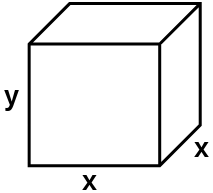
\includegraphics[width=0.2\textwidth]{img/t4.png}
    \end{figure}

    \begin{enumerate}[label=\textbf{\arabic*)}] 
        \item \[\bm{V = x^2y}\]
            \[x^2y = 288\]
            \[y = \frac{288}{x^2}\]

        \item \[\bm{f(x) = 5x^2 + 3x^2 + 3(4xy)} = 8x^2 + 3456x^{-1}\]
            \[f'(x) = 16x - \frac{3456}{x^2}\]
            \[16x - \frac{3456}{x^2} = 0\]
            \[\frac{16x^3 - 3456}{x^2} = 0\]
            \[16x^3 - 3456 = 0\]
            \[16x^3 = 3456\]
            \[x^3 = 216\]
            \[x = \sqrt[3]{216}\]
            \[x = 6\]

        \item 
    \end{enumerate}
\end{document}